\section{Method}
\label{sec:method}

\subsection{Simulating the boot's signal}
Signals are generated at 4\,kHz in the boot's frame ($x$ forward, $y$
lateral, $z$ sole normal) and then passed through the sensor model. The
\emph{gait} is a running stride (2.4--3.2 strides/s): smooth swing-phase
acceleration, a vertical half-sine foot strike (6--14\,g, 25--40\,ms) with a
braking component, foot pitch that rotates gravity in the sensor frame, and
the corresponding angular rate. Three \emph{events} are injected at a random
instant:
\begin{itemize}
\item \textbf{ball}: a half-sine deceleration along $-x$ with peak
  50--130\,g and duration 7--12\,ms \cite{nunome2006impact}, followed by a
  damped 150--260\,Hz ringing at 18\% of the peak;
\item \textbf{player}: an oblique half-sine of 8--45\,g lasting 18--55\,ms,
  followed by a 0.5--3\,g push tail over 60--160\,ms, with a lateral twist on
  the gyroscope;
\item \textbf{both}: a ball pulse and a player pulse separated by a signed gap
  (negative: the player was hit first).
\end{itemize}
Figure~\ref{fig:sig} shows one sampled window of each class.

\begin{figure}[t]
\centering
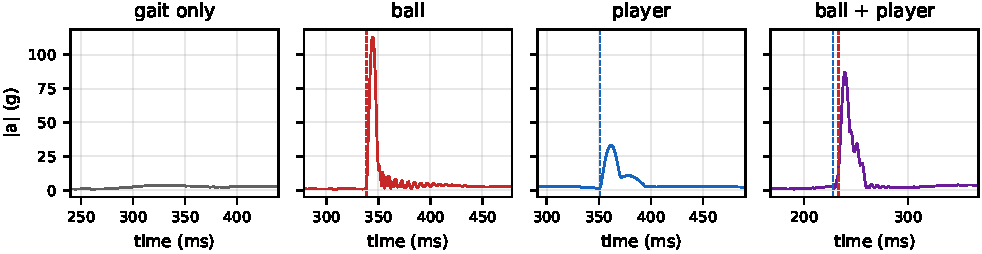
\includegraphics[width=\columnwidth]{figures/signatures.pdf}
\caption{Acceleration magnitude of one window per class at 1\,kHz (impact-rated
sensor). Dashed lines mark the true ball (red) and player (blue) onsets. The
ball is short, hard and rings; the player is longer, softer and pushes; in the
overlap both sit inside one pulse width.}
\label{fig:sig}
\end{figure}

\subsection{Sensor model and real background}
The sensor chain is a first-order low-pass at 45\% of Nyquist, a constant
bias, white noise scaled with $\sqrt{f_s}$, clipping at full scale, and
decimation to the sampling rate $f_s$. Two parts are modelled: an
impact-rated \emph{sport} accelerometer ($\pm200$\,g) and a phone-grade
\emph{consumer} one ($\pm16$\,g). The \emph{ball sensor} reports an impact time
only when the ball is struck, quantised to its 500\,Hz grid with a 1\,ms clock
offset to the boot. As an alternative background we crop real 100\,Hz
ankle-IMU segments of walking, running and playing football from PAMAP2
\cite{reiss2012introducing} (\DetPamSegments\ subject--activity segments) and
inject the same synthetic events; because those recordings contain nothing
above 50\,Hz, the real background is only used at its native rate.

\subsection{Detectors}
\paragraph{Features.} Sixteen pulse descriptors of a window: peak
$|\mathbf a|$ and peak jerk, widths at half and tenth maximum, high-frequency
energy ratio and spectral centroid around the peak, zero crossings of the
post-peak tail (ringing), direction cosines of the peak, gyroscope peaks,
kurtosis, mean of the 40--120\,ms tail (push), background RMS, and the number
of secondary peaks.
\paragraph{Threshold rule.} The connected-ball logic: contact if the peak
exceeds $\tau$; ball if the half-maximum width is below $w$, else player; both
if a second comparable peak exists. $(\tau,w)$ are grid-searched on the
training split, so this baseline is as strong as a threshold rule can be.
\paragraph{Boosting.} Histogram gradient boosting \cite{friedman2001greedy} on
the same features, returning class probabilities.
\paragraph{Onset.} Two estimators anchored on the peak of the \emph{horizontal}
excess (foot strikes are vertical, contacts are not): the first sample above
$\max(6\sigma, 0.08\,\text{peak})$ walking back from the peak, refined by
linear interpolation; and a matched filter on the rising edge of a clean
template with a parabolic sub-sample fit \cite{turin1960introduction}.
\paragraph{Separator.} For the overlap, $|\mathbf a| - \text{baseline}$ is fit
as $A\,T_{\text{ball}}(t-t_1) + B\,T_{\text{player}}(t-t_2)$, $A,B\ge 0$, over a
lag grid, with the closed-form two-column non-negative least-squares solution
\cite{lawson1974solving} vectorised across all $(t_1,t_2)$; a BIC-like penalty
decides whether a second pulse is warranted. The output is the model
(ball/player/both), both onsets, the signed gap and the order.

\subsection{From evidence to a probability}
For a challenge with situation $s$ (standing tackle, sliding tackle, 50/50,
late challenge) the \emph{knowledge base} supplies a base rate
$\pi_s = P(\text{ball first}\mid s)$; the rates used here are illustrative and
are a configuration table. Three sensor sources produce a score in $[0,1]$:
the boosting posterior $P(\text{ball}) + \tfrac12 P(\text{both})$; the
\emph{timing} score $1-\Phi\!\big((\hat t_{\text{ball}} - \hat
t_{\text{boot,first}})/(\sigma\sqrt2)\big)$ from the ball sensor's time against
the boot's first onset, and $0$ if the ball reports nothing; and the
separator's order with confidence $\Phi(|\hat\Delta|/(\sigma\sqrt2))$. Each
score is isotonically calibrated on a held-out half
\cite{zadrozny2002transforming}. Two fusions are compared: the naive-Bayes
log-odds sum $\operatorname{logit}\pi_s + \sum_k
[\operatorname{logit} p_k - \operatorname{logit}\bar p]$, and a stacked
logistic regression on the calibrated log-odds \cite{wolpert1992stacked}. The
\emph{decision} calls ``no foul'' when $P(\text{ball first}) > c_{\text{miss}} /
(c_{\text{false}} + c_{\text{miss}})$, and refers the case to review when the
posterior lies within a band of that threshold.

\subsection{Placing the contact}
A 6-state Kalman filter on position and velocity integrates the world-frame
acceleration obtained from gyro-integrated orientation, with zero-velocity
updates whenever the foot looks planted ($|\boldsymbol\omega| < 40^\circ$/s
and $|\mathbf f| \approx g$) \cite{foxlin2005pedestrian, skog2010zero} and
ultra-wideband position fixes ($\sigma = \LocUwbSigma$\,m) at a configurable
rate. The trajectory is a \LocSpeed\,m/s run with a lateral cut over
\LocDuration\,s; error is scored over the second half of the run. The
probability of misplacing a contact at distance $d$ from a line is
$\Phi(-d/\sigma_{\text{pos}})$.
